% Created 2018-04-18 Wed 13:28
% Intended LaTeX compiler: pdflatex
\documentclass
[
 12pt, % Schriftgröße
       DIV12,
       a4paper,
       oneside,
       titlepage,
       parskip=half,
       headings=normal,
       listof=totoc,
       bibliography=totoc,
       index=totoc,
       captions=tableheading,
       ]{scrreprt}
\input{/Users/dennismuller/dotfiles/networkAssignmentConfig.tex}
\author{Dennis Müller}
\date{\today}
\title{}
\hypersetup{
 pdfauthor={Dennis Müller},
 pdftitle={},
 pdfkeywords={},
 pdfsubject={},
 pdfcreator={Emacs 24.5.1 (Org mode 9.0.5)}, 
 pdflang={English}}
\begin{document}

\tableofcontents


\chapter{Introduction}
\label{sec:org9d46027}

\section{The Idea}
\label{sec:orgb55156f}
A timer tracker app, that can record the spend time on an activity.
To start the activity many there exists many was to activate and deactivate the
time tracker. For example by simply clicking a button, clapping twice, being at
an specifiy geo location, gestures by moving the smartphone around.
Also a separate device (the board) can also be utilized to toggle the time tracker.
Also different activity functions should be able to map to specificy activities
that the user of the app can define on their own.

\section{The Deep Dive}
\label{sec:org697384d}
We want to detect double claps.




\chapter{First Prototype (Board)}
\label{sec:org47f91d8}
Explain the state of what we achieved with the board and what problems arised.
\section{Setup}
\label{sec:orge38cbbc}
\begin{itemize}
\item show board setup
\item some code we used
\end{itemize}



\section{Analysis}
\label{sec:org3a095f8}
\begin{itemize}
\item Diagrams that we had in the presentation. Explain problems.
\end{itemize}

Sample rate to low, memory problems, not so easy to debug ( no way of stepping
through code, no UI for giving fast feedback only LEDs)
\section{Conclusion}
\label{sec:org7d640f8}
move to android.



\chapter{Second Prototype (Android)}
\label{sec:org320397e}
We moved to Android, used the open source Tarsos library that gives us methods to transform
the audio signal from android to FFT.
Higher Samplerates of 20k is not a problems.

\section{Analysis Sound}
\label{sec:org511a6a2}
\begin{itemize}
\item Showing frequence diagrams of recorded tests ( Claps, Husten, Schnippen, Reden)
\item Explain characteristics and approaches for solving the problem of only
detecting the claps.
\end{itemize}

\subsection{Prove that our android FFT works}
\label{sec:org505b32f}
frequenceVonYoutube1200hz.csv

\begin{center}
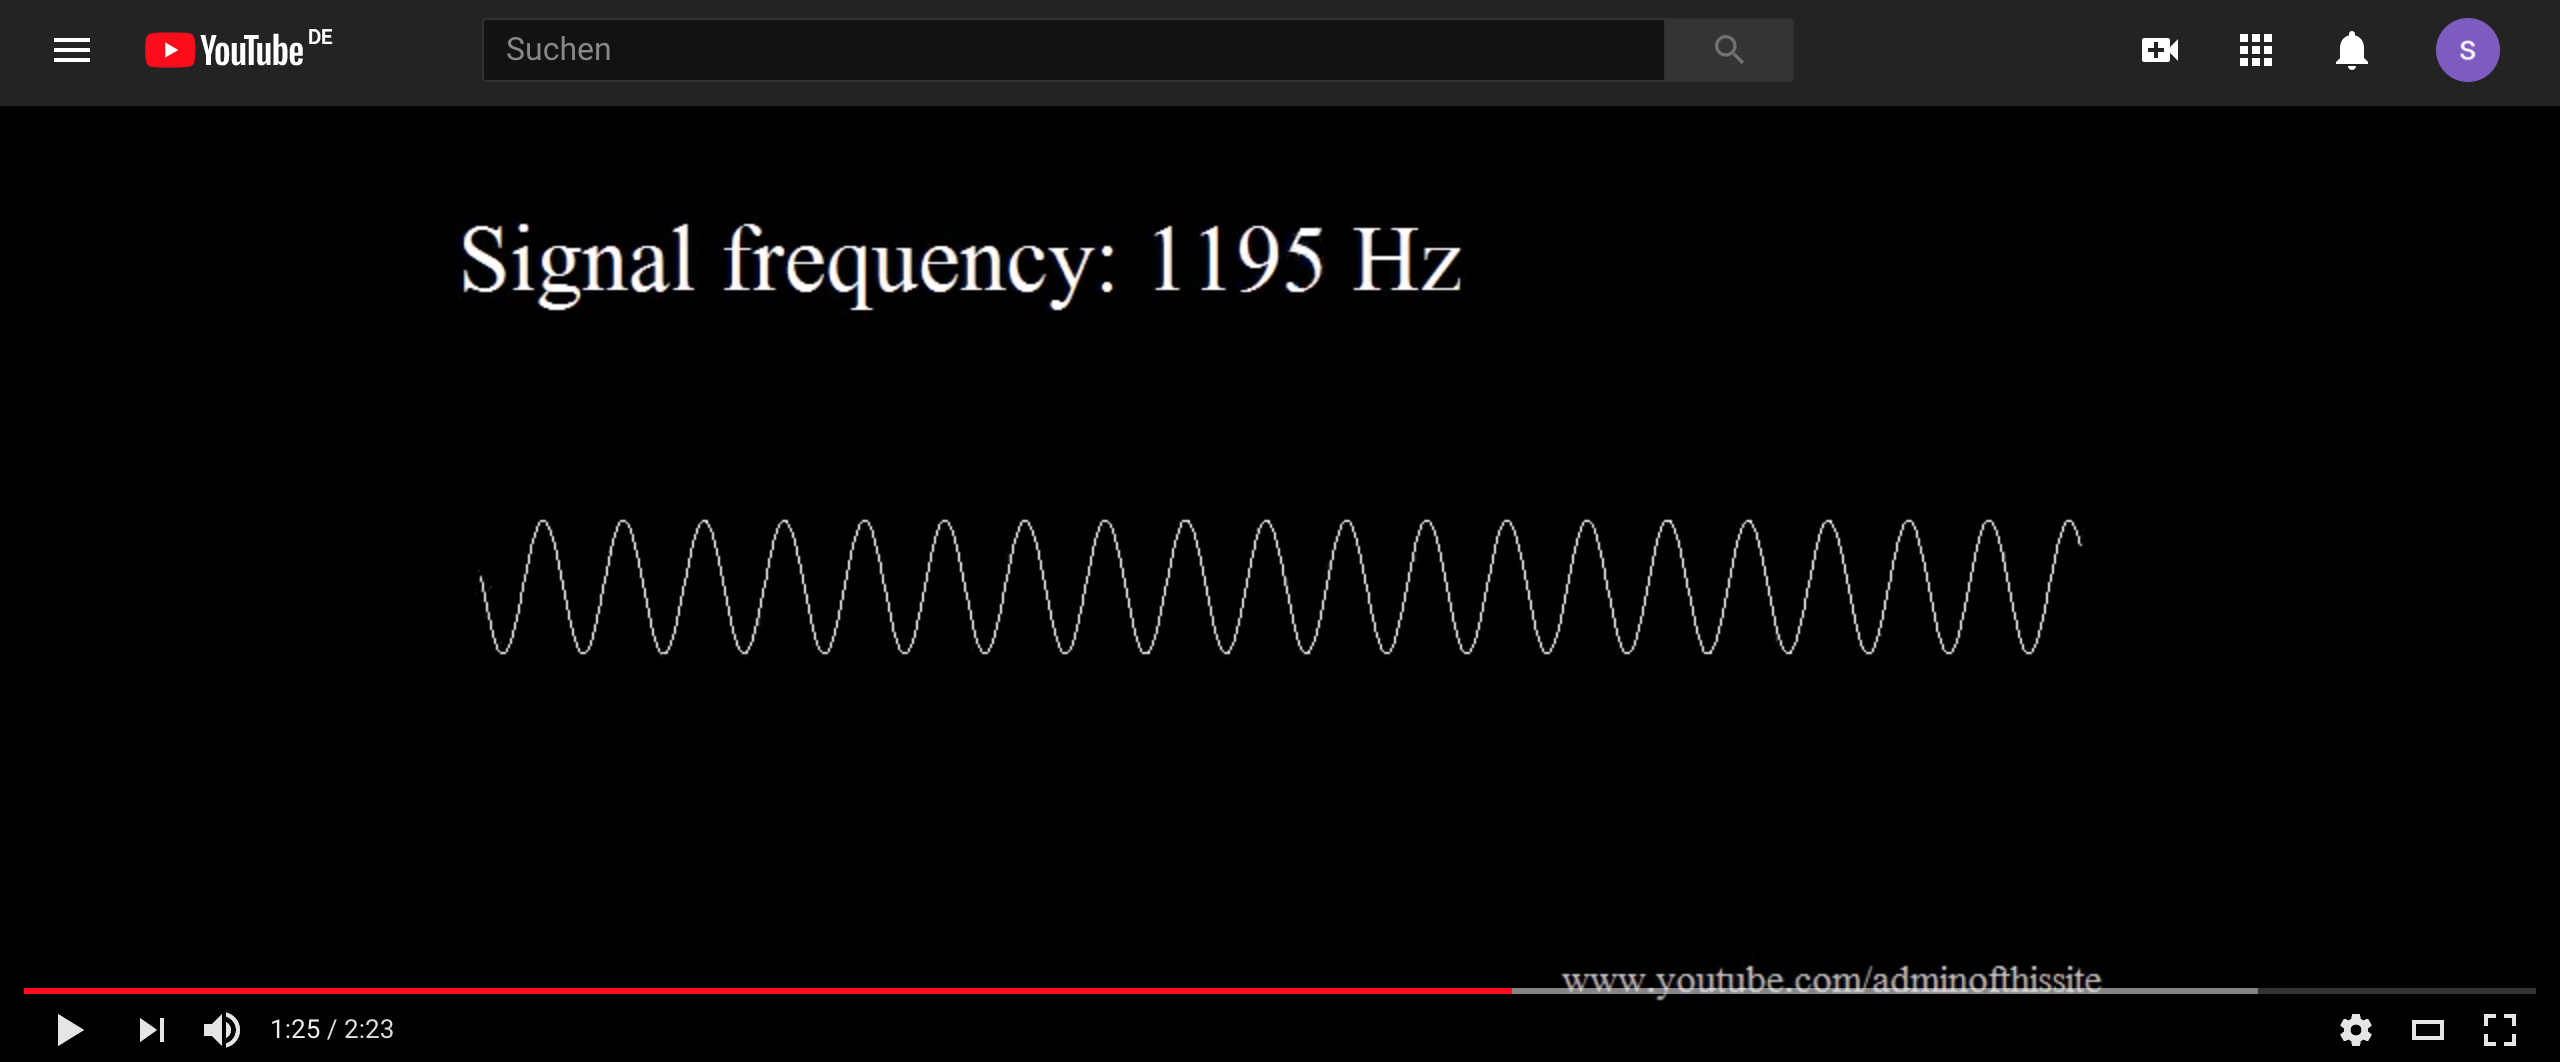
\includegraphics[width=.9\linewidth]{./imgs/ytpicture.png}
\end{center}

\begin{center}
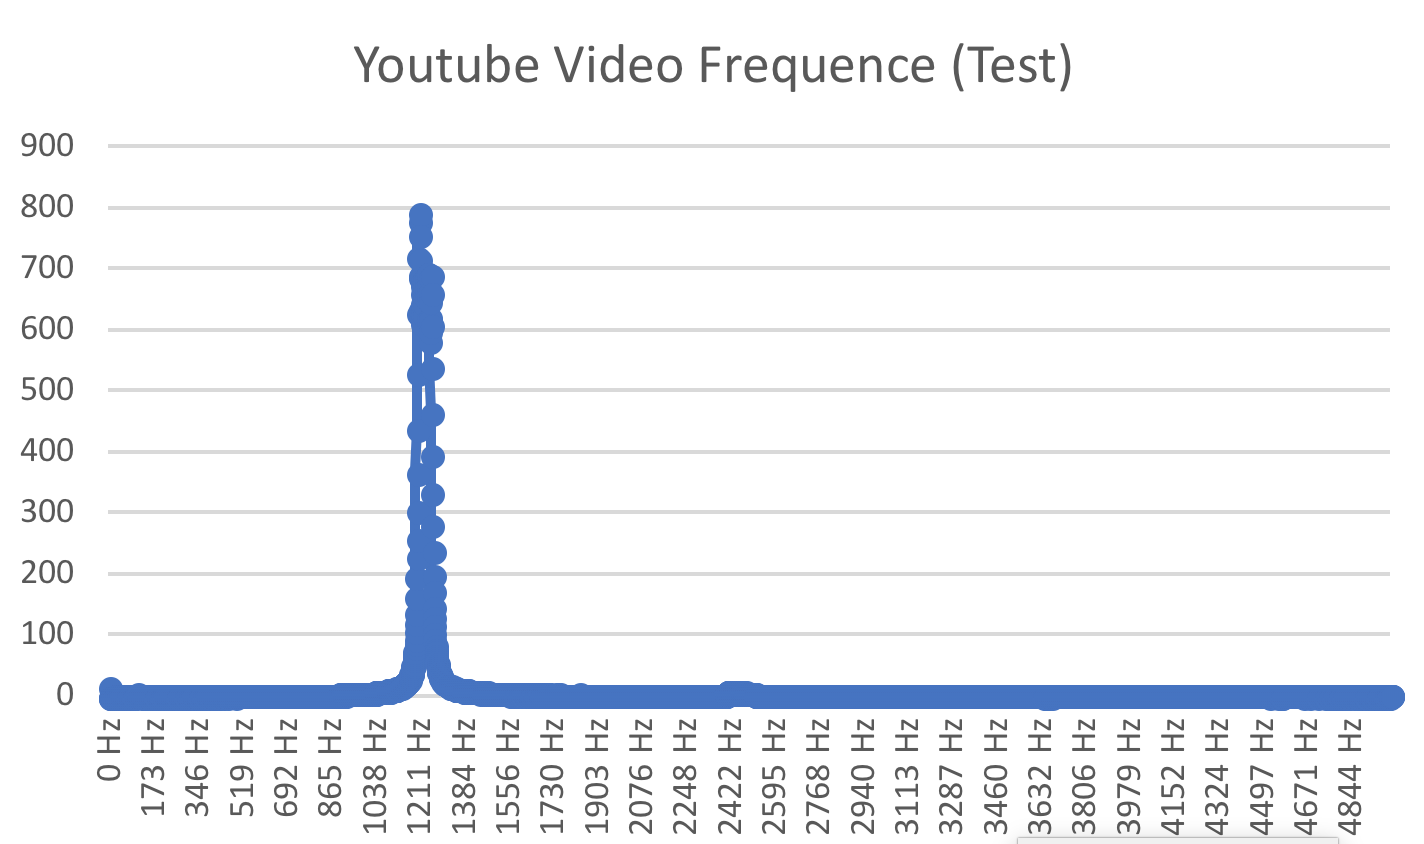
\includegraphics[width=.9\linewidth]{./imgs/yttestandroid.png}
\end{center}

\url{https://www.youtube.com/watch?v=qNf9nzvnd1k}

\chapter{Implementation (Android)}
\label{sec:org1401e45}
\begin{itemize}
\item UI Screenshots
\item How we implemented the clap detection in the end.
\end{itemize}

\section{Evalutation}
\label{sec:orge1bedac}
\begin{itemize}
\item How reliable can our implementation detect clap.
\item Show statistics by trying it out (maybe in different environments (loud,
silent rooms, outdoors)
\end{itemize}

\chapter{Conclusion}
\label{sec:org77e7451}
\section{Current State}
\label{sec:orgc960a3e}
Refer to to evalution part above. State how difficult this was and the time
needed to try out more advanced solutions (AI) was not enough.

\section{Project Future}
\label{sec:orgeb9e4a8}
Maybe add more debug functionallity inside the App, be able to not only tweak
parameters inside the code, but also with UI Controls inside the app.



\chapter{Referernces}
\label{sec:orgdc7d373}
\url{http://www.klangfuzzis.de/showthread.php?679817-Was-hat-in-etwa-wie-viel-hz}
\end{document}